\section{基本放大电路}
        \begin{figure}[H]
            \centering
            
\includegraphics[width=7cm]{img/2.0.png}
            \end{figure}
是\underline{\textbf{功率}}放大,本质上还是能量控制和放大,必要条件是要有有源元件,前提是不失真,用\underline{\textbf{正弦波}}测试。

\subsection{怎样构建(基本放大电路)}
我们只有一个小功率信号,元件,电源。让晶体管工作在\underline{\textbf{放大}}区,小信号需要控制$i_B$,实际上是控制
$U_{BE}$。
        \begin{figure}[H]
            \centering
            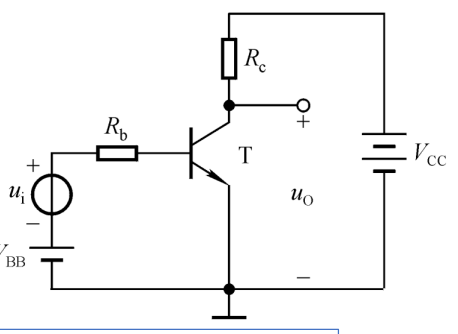
\includegraphics[width=7cm]{img/2.1.png}
            \end{figure}
首先是正反偏,然后输入加入电阻保护,加上输出电阻输出电压。
\begin{description}[leftmargin=0.9cm,style=nextline,nosep]% nosep没有垂直间隔
    \item[$V_{BB}$] 抬高小信号电压,使三极管发射结正偏。
    \item[$V_{\mathbb{C}}$] 使得三极管集电结反偏。
    \item[$R_b$] 保护。
    \item[$R_c$]  使得输出电压。
    \item[$u_i$] 输入电压     
    \item[静态工作点$Q$] $u_i=0$的时候,此时各个参数的表示为$I_{BQ},I_{CQ},U_{BEQ},U_{CEQ}$ 。
    \item[静态工作点的必要性] 因为要解决失真问题,使三极管工作在线性区,使信号不失真。  
\end{description}

% \subsubsection{共射放大电路}
对于共射放大电路,负载上无直流份量,也可以在输入或者输出加上\underline{\textbf{耦合电容}}来隔离\textbf{直流},通过交流,叫做阻容耦合电路。
% \subsection{分析方法}
我们按照过程(电容耦合下),有如下
\begin{align}
u_{BE}&=u_i \tag{3.1.a}\\
i_{B}&=\frac{u_{CC}-u_{BE}}{R_{B}} \tag{3.1.b}\\
i_{C}&=\beta i_{B} \tag{3.1.c}\\
u_{CE}+R_Ci_C&=u_{CC}    \tag{3.1.d}
\end{align}
\subsubsection{性能参数}
\begin{figure}[H]
    % \centering
    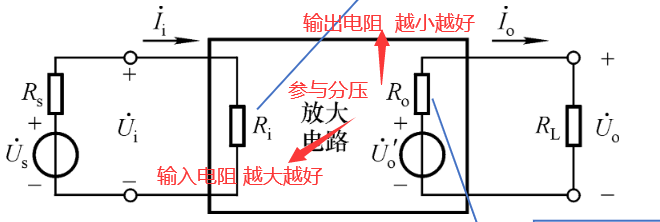
\includegraphics[width=7cm]{img/2.3.png}
    \end{figure}
    
任何一个放大电路都可以看作是一个二端口网路,定义放大倍数为输入和输出量之比,但是电压放大倍数$\dot{A_{uu}}$是最常被研究的
通频带
\begin{figure}[H]
        % \centering
        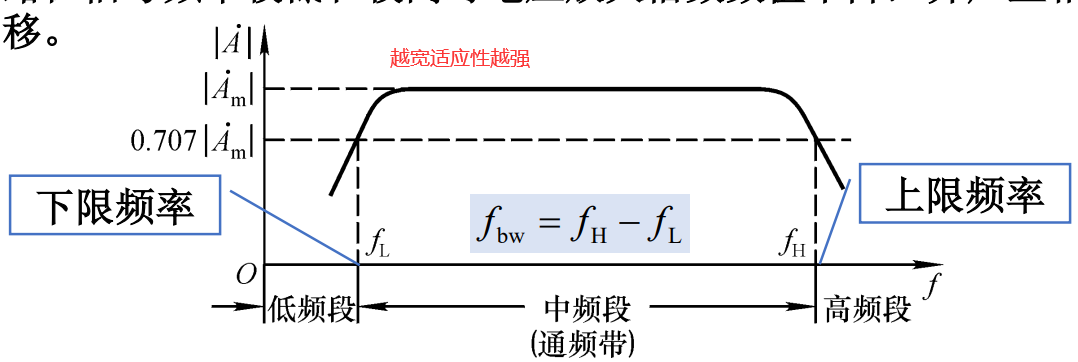
\includegraphics[width=7cm]{img/2.2.png}
        \end{figure}

\begin{definition}[非线性失真系数]
$$
D=\frac{\sqrt{\sum_{i=1}^{\infty}{U_{i+1}^2}}}{U_1}
$$
\end{definition}
最大输出功率$p_{om}$,电源效率为$\eta=\frac{p_{om}}{p_v}$
\subsubsection{直流通路和交流通路}
\begin{description}[leftmargin=1.7cm,style=nextline,nosep]% nosep没有垂直间隔
    \item[直流通路] $U_S=0$,电容开路,电感短路。用于研究静态工作点
    \item[交流通路] 直流电源短路,大容量电容短路。  用于动态参数研究
\end{description}

先静后动。静态有计算和图解,动态有图解和微变等效。
\subsection{静态分析方法}

\subsubsection{图解法}
在三极管的输入和输出曲线上,画出外部的工作线。
        \begin{figure}[H]
            \centering
            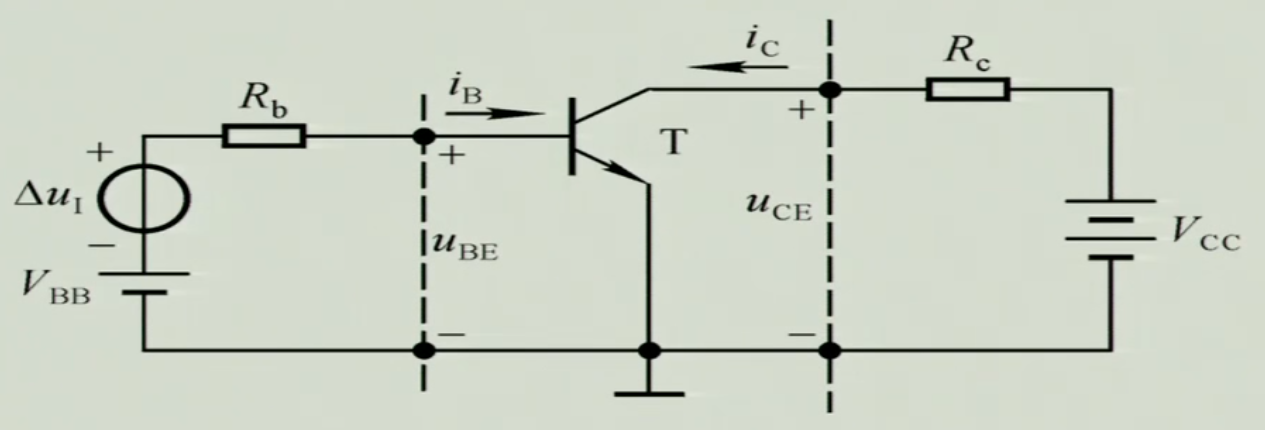
\includegraphics[width=7cm]{img/2.4.png}
            \end{figure}
\begin{align}
i_b=\frac{V_{BB}-U_{BE}}{R_b} \tag{3.1.a} \\
i_c=\frac{V_{CC}-U_{CE}}{R_c} \tag{3.1.b} 
\end{align}
(3.1.a)是对于输入曲线,(3.1.b)对于输出曲线。纵坐标是
$\displaystyle  \frac{V_{\mathbb{CC}}}{R_c}$,
横坐标是$V_{CC}$,对于放大倍数,有如下:
        \begin{figure}[H]
            \centering
            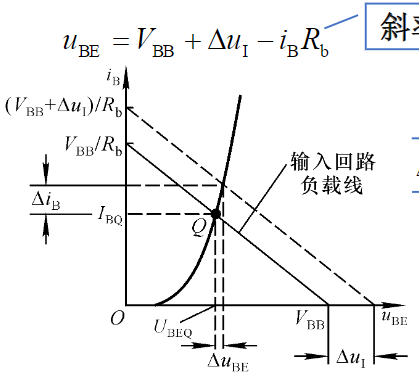
\includegraphics[width=7cm]{img/2.5.png}
            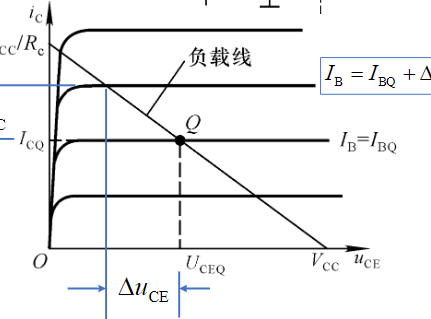
\includegraphics[width=7cm]{img/2.7.png}

            \end{figure}
\subsubsection{电位分析法}
一个一个地写起来,使用基尔霍夫电压定律。
\subsubsection{估算法}
本质是两个直线相交。利用$U_{BEQ=0.7V}$
        \begin{figure}[H]
            \centering
            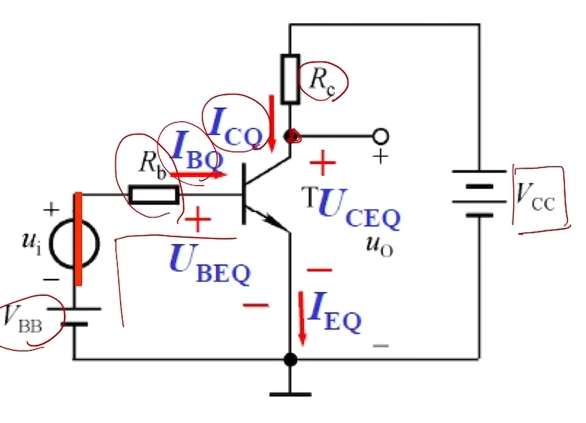
\includegraphics[width=7cm]{img/2.8.png}
            \end{figure}
\begin{align}
    V_{BB}=R_bI_{BQ}+0.7 \tag{3.2.a} \\
    I_{B_Q}:I_{CQ}:I_{EQ}=1:\beta:1+\beta\tag{3.2.b}
\end{align}

\subsubsection{等效电路}
先找Q点,再找$\displaystyle r_{be}=r_{bb}+(H\beta)\frac{U_T}{I_{EQ}}$

\subsubsection{静态分析法列写方程}

\subsection{动态分析}
\subsection{h参数等效电路}
中低频,小信号。
\subsubsection{三极管的等效模型}
三极管可以简化成一个h参数微变等效模型

\begin{figure}[H]
            \centering
            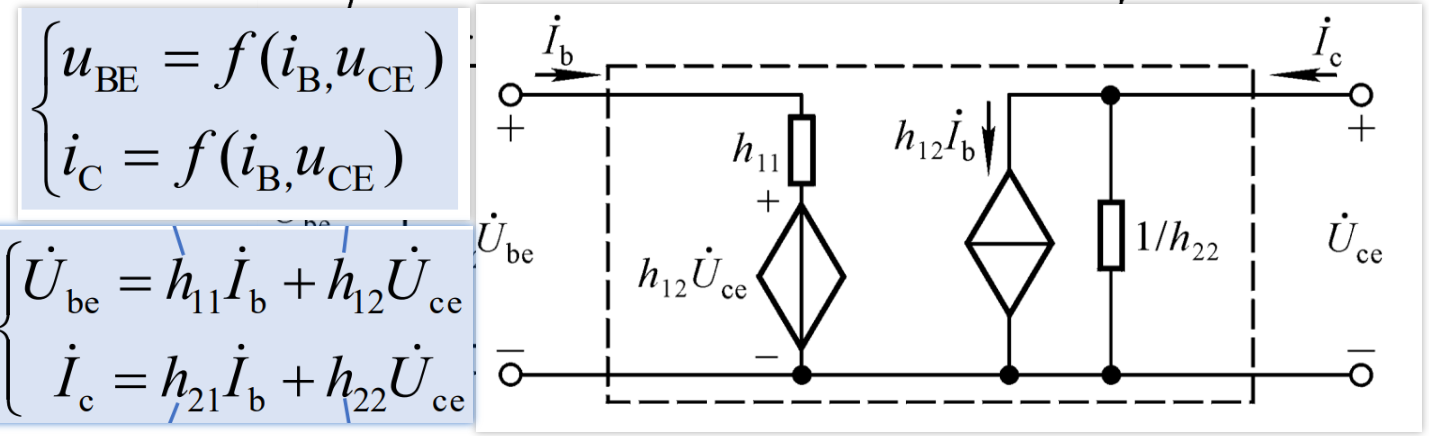
\includegraphics[width=8cm]{img/2.9.png}
            \end{figure}
并且一般的来说有如下
\begin{align}
 h_{11}=r_{be}\thickapprox 0\tag{3.3.a} \\
 h_{12}=\frac{\Delta_{BE}}{\Delta_{CE}}\tag{3.3.b} \\
 h_{21}=\beta\thickapprox \infty\tag{3.3.c} \\
 h_{22}=\frac{1}{r_{ce}}\tag{3.3.d} 
\end{align}
继续简化就可以得到
\begin{figure}[H]
    \centering
    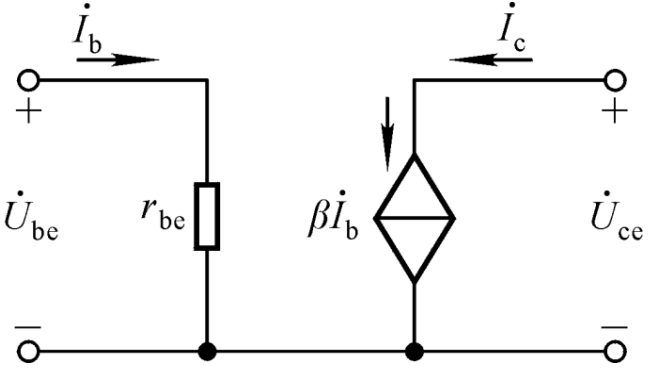
\includegraphics[width=7cm]{img/2.10.png}
    \end{figure}
并且有$r_{bb'}$ 为基区体积电阻,$r_{b'e}$为发射结微分电阻,$r_{ce}$为集电结微分电阻,$U_T=26(mV)$。
\begin{figure}[H]
    \centering
    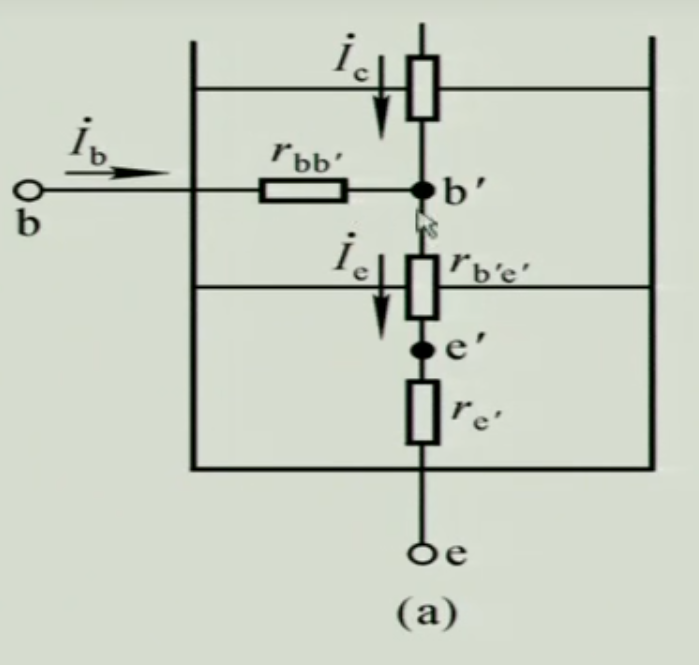
\includegraphics[width=7cm]{img/2.12.png}
    \end{figure}
$$ 
\begin{aligned}
    U_{be}&=I_b(r_{bb'})+I_{e}(r_{b'e}) \\
    r_{be}&=\frac{U_{be}}{I_b}=r_{bb'}+r_{b'e}
    \\&=r_{bb'}+(1+ \beta)\frac{U_T}{I_{EQ}(mA)} 
    \\&=r_{bb'}+\frac{U_{T}}{I_{BQ}}
\end{aligned}
$$
\subsubsection{直接接法}
之前等效的左b右c下e。VCC对交流短路,所以可直接当接地。具体如下图
        \begin{figure}[H]
            \centering
            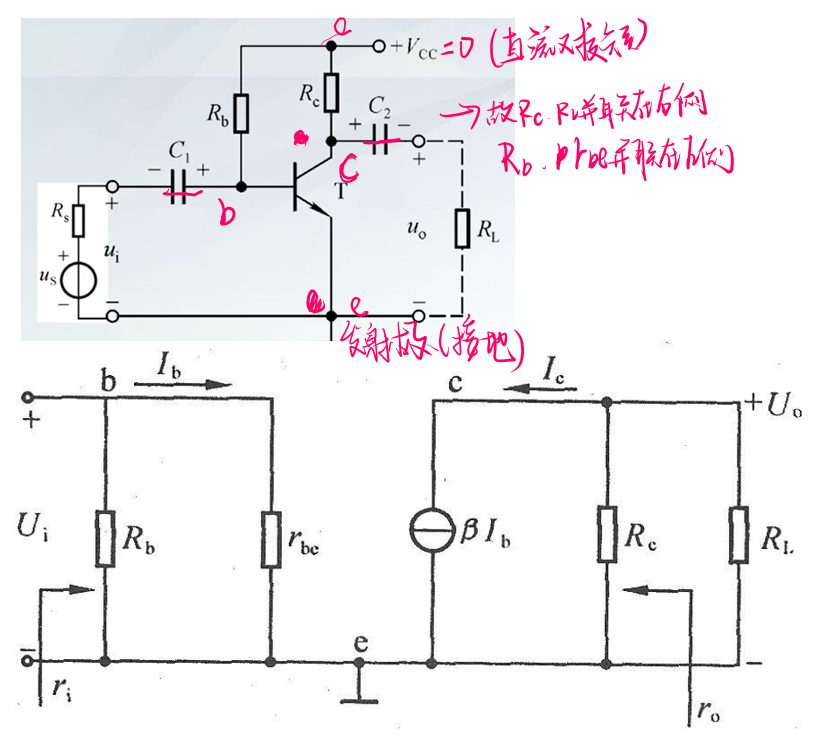
\includegraphics[width=7cm]{img/2.11.png}
            \end{figure}
下面计算一些常用参数
\begin{align}
    A_{u}&= \frac{U_{o}}{U_{i}}= \frac{-i_{c}R_{o}}{i_{b}r_{be}}=- \frac{\beta R_{o}}{r_{be}} \tag{3.4.a} \\
    R_i&=\frac{U_i}{I_i}=R_b // r_{be} \tag{3.4.b}\\
    R_o&=\frac{U_o}{I_o}=R_c // R_L\thickapprox R_c \tag{3.4.c}\\
    r_{be}&=r_{bb'}+\frac{U_T}{I_{BQ}} \tag{3.4.d}\\
    A_I&\thickapprox \beta \frac{R_{L}'}{R_L}
\end{align}
\subsubsection{最大不失真电压}
\subsubsection{失真分析}
\subsection{放大电路Q点的稳定性}
温度,电源波动,元器件老化都会引起Q点波动。会失真,截至失真,饱和失真。
\subsubsection{如何稳定}
所谓Q点稳定,是指$ I_{CQ} $ 和 $ U_{CEQ} $在温度变化时基本不变,
这是靠$ I_{BQ} $的变化得来的(加了反馈电阻$R_e$)。
        \begin{figure}[H]
            \centering
            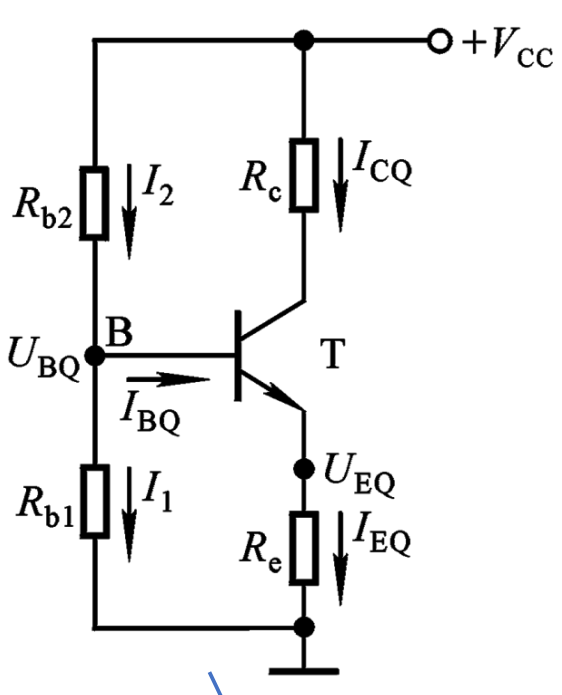
\includegraphics[width=5cm]{img/2.13.png}
            \end{figure}

